% This syllabus template was created by:
% Brian R. Hall
% Assistant Professor, Champlain College
% www.brianrhall.net

% Document settings
\documentclass[11pt]{article}
\usepackage[margin=1in]{geometry}
\usepackage[pdftex]{graphicx}
\usepackage{multirow}
\usepackage{setspace}
\usepackage{listings}
\pagestyle{plain}
\setlength\parindent{0pt}

\begin{document}
	
	 
	\section*{Les diagrammes thermodynamiques}
	
	Leur but principal est de rassembler, dans un seul document, de nombreuses informations concernant les gaz réels (lorsqu’on ne peut plus appliquer les lois du gaz parfait).
	
	\begin{itemize}
		\item Diagramme pression-volume (P-V) : utilisé pour étudier les transformations (compression, détente). Le travail effectué peut être calculé comme la surface sous la courbe de transformation.
		
		\item Diagramme température-entropie (T-s) : permet de visualiser les échanges de chaleur. La chaleur échangée peut être calculée comme la surface sous la courbe.
		
		\item Diagramme de Mollier (h-s)
		
		\item Diagramme enthalpique (h-p), parfois aussi appelé diagramme de Mollier.
	\end{itemize}
	
	\subsection*{Diagramme de Mollier}
	
	Le diagramme de Mollier représente l'enthalpie $h$ en fonction de l'entropie $s$. Il est utilisé notamment pour la vapeur d'eau et les cycles frigorifiques.
	
	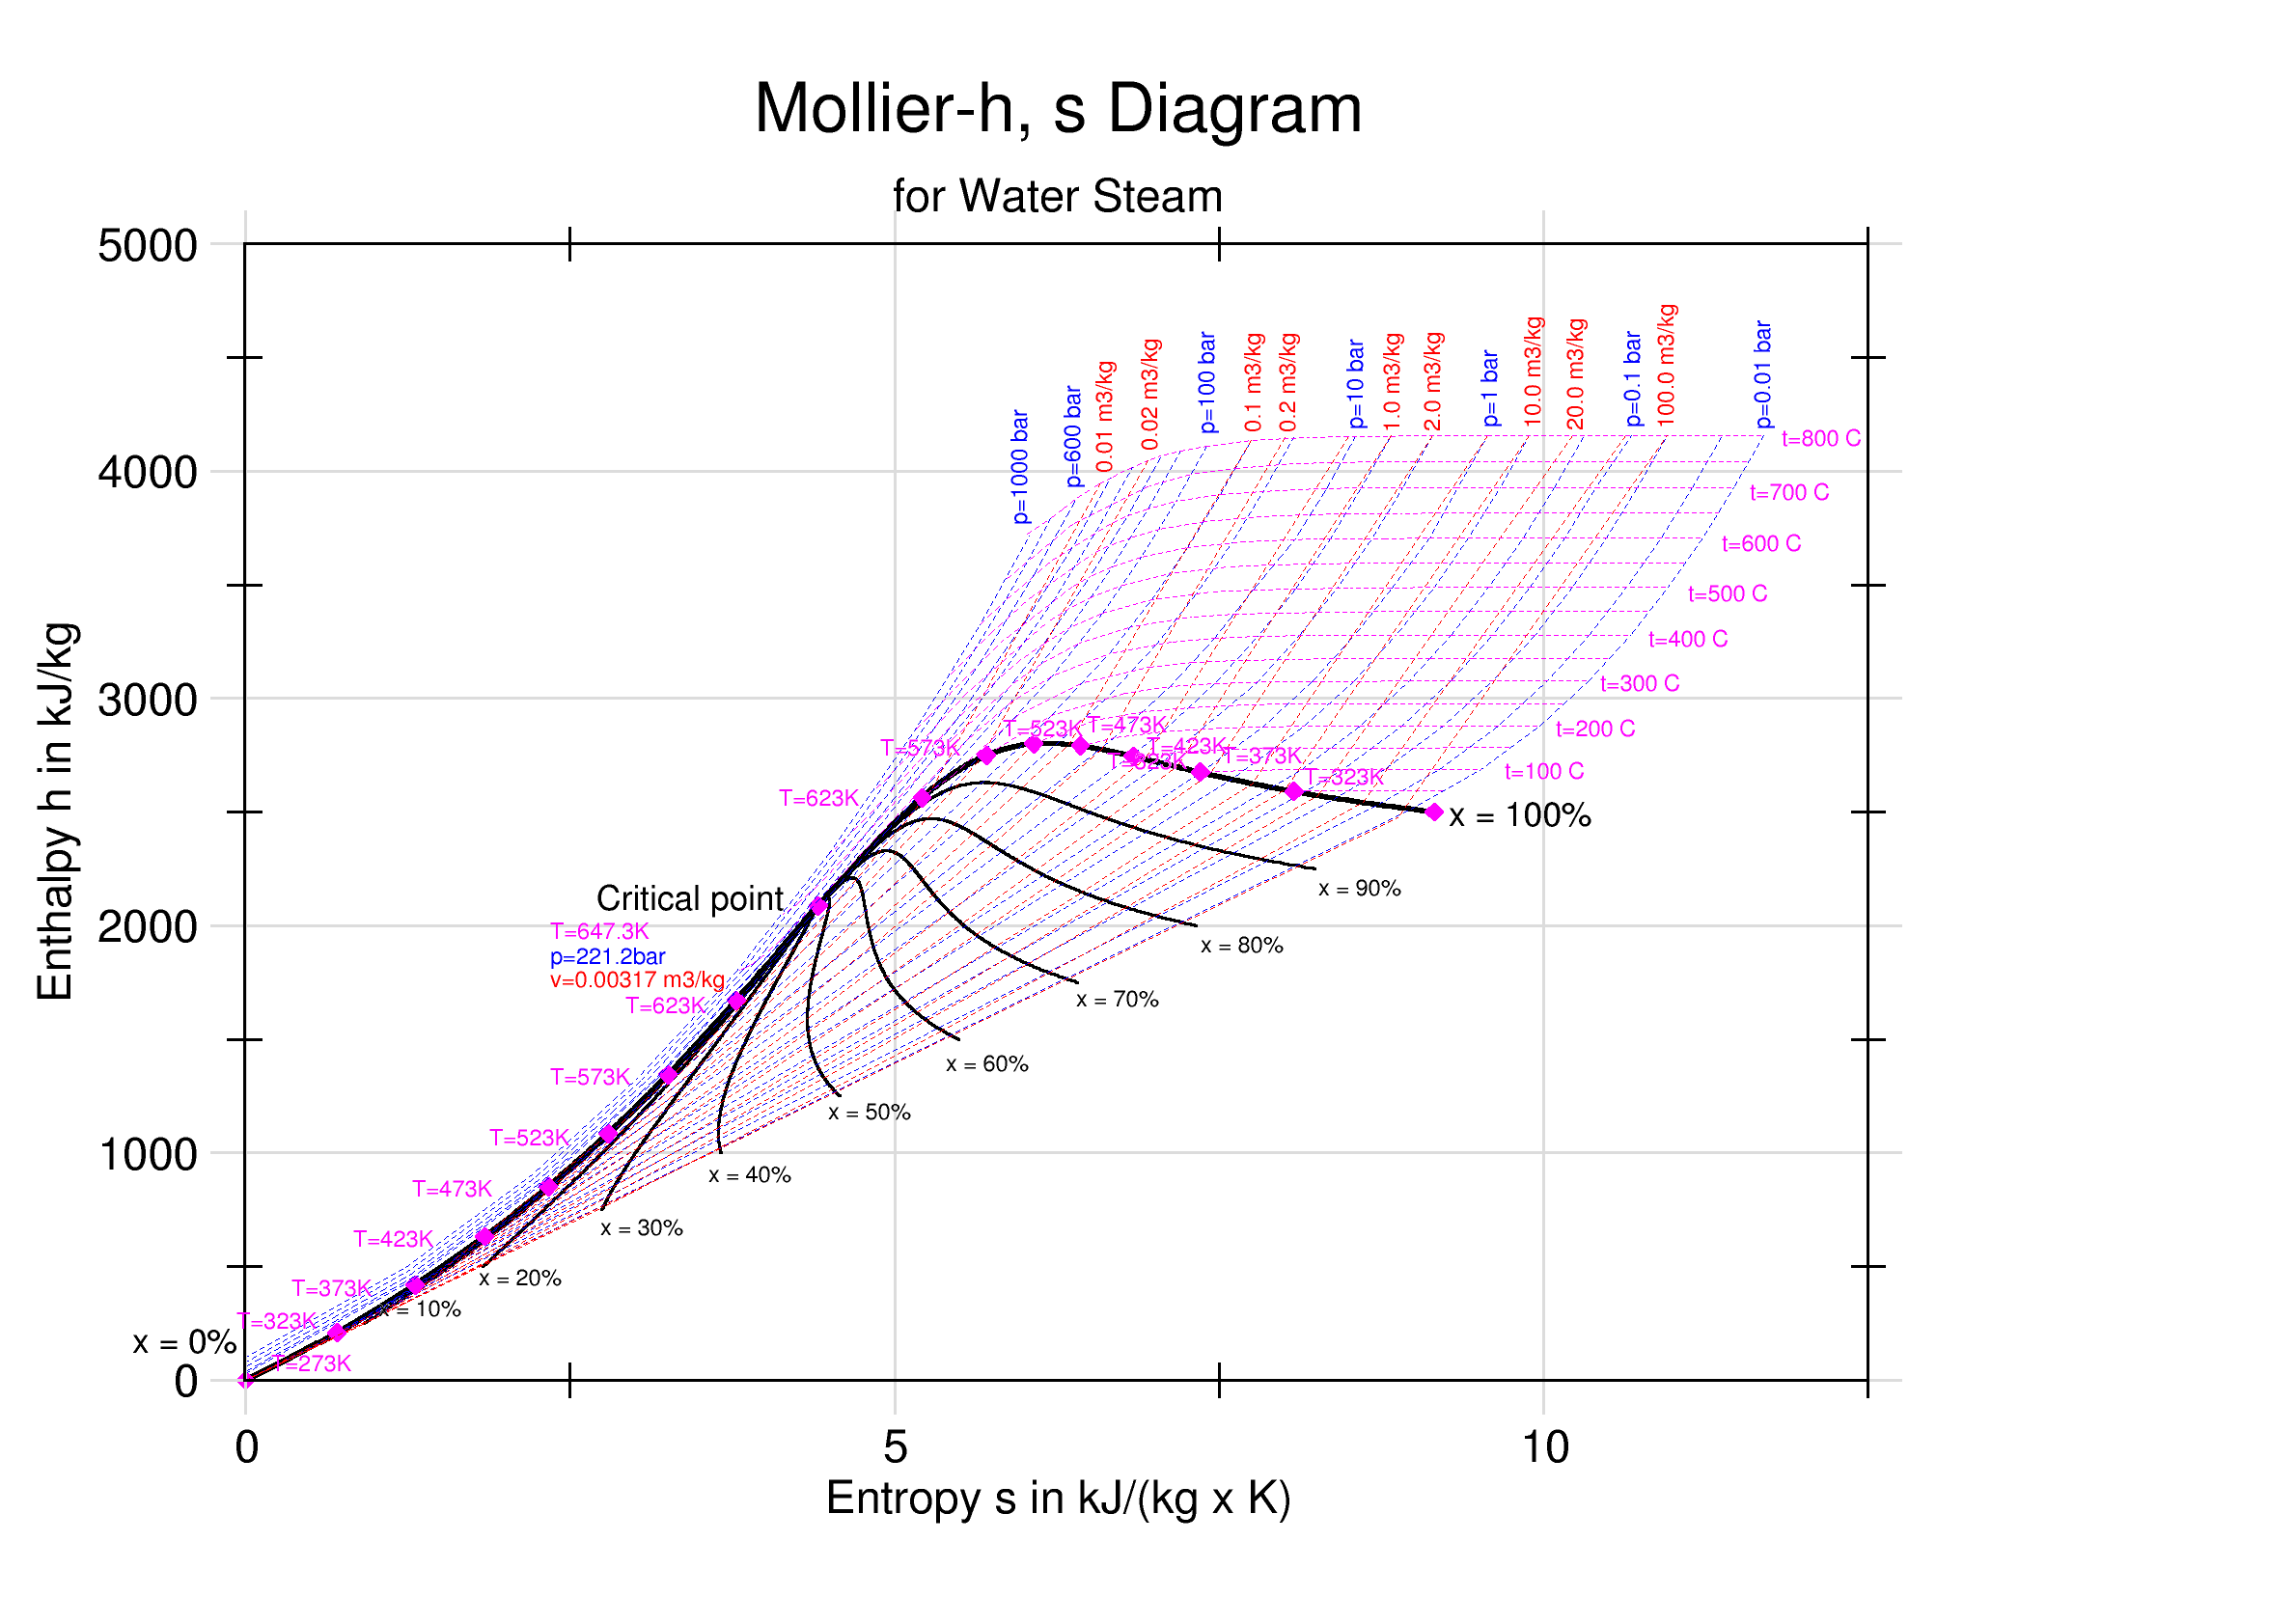
\includegraphics[width=0.7\linewidth]{images/diag_complete.png}
	
	On y trouve :
	\begin{itemize}
		\item les isobares (pression constante)
		\item les isothermes (température constante)
		\item le titre de vapeur $x$
		\item les zones liquide, vapeur et mélange
	\end{itemize}
	
	\subsubsection*{Remarque 1}
	Dans la zone de mélange liquide-vapeur, une pression constante correspond à une température constante. La chaleur ajoutée ou enlevée sert à modifier la proportion de liquide et de vapeur.
	
	\subsubsection*{Remarque 2}
	À pression constante :
	\[
	\Delta H = \Delta U + P \Delta V = \Delta Q
	\]
	
	À température constante pour un procès réversible:
	\[
	T \Delta S = \Delta Q
	\]
	
	On en déduit que :
	\[
	T \Delta S = \Delta H
	\]
	
	Ainsi, les lignes isobares sont des droites dans la zone de mélange liquide-vapeur.
	
	\subsubsection*{Exemple : turbine à vapeur}
	Sera étudié dans le TD4.
	
\end{document}
 
 



